The \gtx{} algorithm takes as input an unweighted graph topology $G_0=(V_0, E_0)$ and produces a sequence of
graphs $\{G_t\}_{t=1}^T$ of decreasing size until each connected component of $G_0$ is reduced to a
single node. As we will prove later, after reaching this point, the algorithm has selected $|V_0| -
1$ edges that form a spanning tree of $G_0$. Intuitively, $G_{t+1}$ is obtained from $G_t$ by composing two
primitives so that we can informally write $G_{t+1} = \left(\contractStar{} \circ
\extractStar{}\right)(G_t)$.

\extractStar{} partitions the graph $G_t$ into a set of stars and \contractStar{} build the graph
made of those stars using the edges in $E_t$. We provide more details on those two operations in the
following, as well as their complexity analysis. Then we state formally the \gtx{} algorithm and prove
its termination and correctness.  Finally, we study its properties, such as the number of iterations
needed to finish and the stretch of the resulting tree. For simplicity and without loss of
generality, we assume that $G_0$ through $G_T$ consist of a single connected component.

\medskip

\paragraph{\extractStar{}}\label{par:extractstar}%
\extractStar{} takes as input a graph $G_t=(V_t, E_t)$, and optionally a \emph{threshold function}
$t_f$ or a \emph{degree function} $d_f$. While the nodeset $V_t$ is not exhausted, it repeatedly samples a
node $c_i$, creates a star $S_i^t$ with $c_i$ at its center and the neighbors of $c_i$ on the
periphery, removes all the nodes of $S_i^t$ from
$V_t$ and all the edges incident to $S_i^t$ from $E_t$, and finally decrements accordingly the
degree of the 2-hop neighbors of $c_i$ (see \autoref{fig:gtx_star_simple} for a visual
representation of this notation).
\begin{marginfigure}
  \centering
  \includegraphics[height=0.15\textheight]{assets/tikz/gtx_star_tikz.pdf}
  \caption[A sample star]{A sample star created during the \tth{} contraction level. The black node
    % \tikz{\node[vertex,rare] {$c_i$};}
    is the center $c_i$ of the star $S_i^t$, which is also made of the four light gray peripheral nodes
  % \tikz{\node[vertex,medium] {$p_1$};} to \tikz{\node[vertex,medium] {$p_4$};}
  as well as the solid edges. The 2-hops neighbors of $c_i$ are the white nodes
  % \tikz{\node[vertex] {$h_1$};} to \tikz{\node[vertex] {$h_3$};}
  $h_1$ to $h_3$, whose degree will decrease once $S_i^t$ is removed from $G_t$.}
  \label{fig:gtx_star_simple}
\end{marginfigure}%
Upon completion, it returns a list of stars and a mapping of
each node of $V_t$ to the unique star it belongs to. We consider three heuristics to sample centers:

\begin{itemize}%[nosep]
  \item choose the node with the current highest degree, with ties broken arbitrarily
  \item if $n_i$ is the number of node remaining in $V_t$ before choosing the \ith{} center, choose
    a node \uar{} among those with a degree larger than $t_f(n_i)$. Setting the threshold function
    to be the identity therefore recovers the previous strategy, but the idea here is to choose
    among a small set of high degree nodes, for instance by letting $t_f(n) = \sqrt{n}$
  \item if $\degr_i(u)$ is the degree of node $u$ before iteration \ith{}, choose node
    proportionally to $d_f(\degr_i(u))$.  Again, the degree function is designed so that it favors the
    selection of high degree nodes. For instance, one could use $d_f(\degr_i(u)) = \degr_i(u)^2$.
\end{itemize}

We now give the pseudo code of \extractStar{} for the highest degree variant.\footnote{Note that for
clarity, we removed some bookkeeping code in all listings, mainly the part related to maintaining
mapping between nodes at different level of contraction. However, the full python implementation
is available at \url{https://github.com/daureg/magnet/blob/master/veverica/new_galaxy.py\#L27}.}
We assume that $G$ is the adjacency list of the graph, so that $G[u]$ is the set of neighbors of
$u$, \ie{} $G[u] \equiv \mathcal{N}(u)$. The other piece of notation is $\textsc{Star}$, which
simply create a star given a center and a list of peripheral nodes.  \vspace{-\baselineskip}

\begin{center}
  \rule{\textwidth}{.3pt}
  \begin{algorithmic}[1]
    \Function{\extractStar{}}{$G_t=(V_t,E_t)$}
      \State Let $Q$ be a max-priority queue. The key of element $x$ is $Q[x]$
      \Let{$stars$, $inner\_edges$, $remaining$}{$[]$, $\emptyset$, $\emptyset$}
      \ForAll{node $u$ in $V_t$}
        \State \Call{Insert}{$Q,\,u$} \Comment with the key $\degr(u)$
        \Let{$remaining$}{$remaining \bigcup \left\{u\right\}$}
      \EndFor
      \While{$Q$ is not empty}
        \Let{$c_i$}{\Call{Extract-Max}{$Q$}}
        \If{$c_i$ not in $remaining$}
          \State \textbf{continue} \Comment{$c_i$ is part of an existing star so there is
          nothing to do}
        \EndIf
        \Let{$periphery$}{$G[c_i] \bigcap remaining$}
        \Let{$stars$}{$stars \bigcup \{$\Call{Star}{$c_i,\, periphery$}\}}
        \Let{$inner\_edges$}{$inner\_edges \bigcup \{(c_i, p): p \in periphery\}$}
        \Let{$remaining$}{$remaining \setminus\left\{c_i\right\} \setminus periphery$}
        \For{$p$ in $periphery$}
          \For{$h$ in $G[p] \bigcap remaining$}
            \State \Call{Decrease-Key}{$Q,\, h,\, Q[h]-1$}
          \EndFor
        \EndFor
      \EndWhile
      \State \textbf{return} $stars$, $inner\_edges$, $membership$%
      \Comment{$membership$ maps the nodes of $V_t$ to the index of the star they belong to}
    \EndFunction
  \end{algorithmic}
  \rule{\textwidth}{.3pt}
\end{center}

\extractStar{} terminates because at each iteration of the while loop line 8, we remove one node
from $Q$ and never add any. Let us analyze the complexity when $|V_t|=n$ and $|E_t|=m$. We first
build a priority queue of all the nodes sorted by their degree (line 5--7), which takes $O(n)$ time.
Then, at each iteration of the inner loop, we find the center of the next star by extracting the
maximum of the queue (line 9), we build the corresponding star (line 12--14) and we decrease the
priority (\ie{} the degree) of all nodes adjacent to the new star (line 15--17).  Since both
operations require constant time when using a Strict Fibonacci Heap~\autocite{FibonacciHeaps12} and
there are $n$ iterations of that loop, a coarse approximation of the runtime of \extractStar{} is
$O(n^2)$. However, observe that there can be at most $m$ decrease operations (since after that, all
nodes still in the queue have an effective degree of $0$, meaning that $periphery$ will the empty
set and lines 13--17 will run in constant time), reducing the complexity to $O(m+n)$.

The other two variants are more time consuming because they require additional bookkeeping. Their
randomization make them useful in an adversarial context but it also renders the analysis  of the
resulting spanning tree more challenging\marginpars{Which means this paragraph can be skipped at first.}
Therefore, we only briefly describe the implementations here.\footnote{Although they are available
online at 
\nolinkurl{https://github.com/daureg/magnet/blob/master/veverica/}%
\{\href{https://github.com/daureg/magnet/blob/master/veverica/ThresholdSampler.py}%
{ThresholdSampler.py}, \href{https://github.com/daureg/magnet/blob/master/veverica/NodeSampler.py}%
{NodeSampler.py}\}.} For the threshold function, we
maintain two queues, $high$ and $low$, containing nodes whose degree is respectively above and below
the current threshold. We select a node \uar{} in $high$, remove the corresponding star from $G_t$,
recompute the new threshold and if necessary, move nodes which fell under the threshold from $high$
to $low$ and those who climb above the threshold from $low$ to $high$. For the degree function, we
can draw any node as center proportionally to its weight (where the weight of node $u$ is defined as
$d_f\left(\degr(u)\right)$). Yet we cannot use the standard method of computing the cumulative sum
of weights since some of them change at each iteration. Therefore, we construct a binary tree whose
leaves are the nodes of $V_t$ and where each tree nodes maintain the sum of weights in its left and
right subtrees. To sample, we draw a random number $r$ between $0$ and the total weight of the tree and
go down from the root to the leaf spanning the weight interval containing $r$.
When degrees are updated (or graph node removed), we update the weights along a path from the
corresponding leaves to the root of the tree.

\medskip

\paragraph{\contractStar{}}\label{par:contractstar}%
The second routine, \contractStar{} takes as input the result of \extractStar{}, along with $E_t$
and an optional $\emph{eccentricity}$ array we will describe soon\marginpars{Actually, we could make
eccentricity the default behavior, which would simplify the pseudo code}. It builds a new graph $G_{t+1}$
where each star becomes a node and where there is a link between two nodes $s_1$ and $s_2$ if the nodes
making up $s_1$ and $s_2$ are connected in $E_t$.

\begin{center}
  \rule{\textwidth}{.3pt}
  \begin{algorithmic}[1]
    \Function{\contractStar{}}{$E_t,\,membership,\,eccentricity$}
      \State Let $G_{t+1}$ be an empty graph
      \State Let $cross\_edges$ be a mapping from edges in $G_{t+1}$ to set of edges in $G_t$
      \ForAll{edge $(u, v)$ in \Call{Shuffle}{$E_t$}}
        \Let{$s_u,\,s_v$}{$membership[u]$, $membership[v]$}%
        \Comment{swap if needed so that $s_u < s_v$}
        \If{$s_u = s_v$}
          \State \textbf{continue}
        \EndIf
        \If{$eccentricity$ is not \textbf{null}}
          \Let{$cross\_edges[(s_u, s_v)]$}{$cross\_edges[(s_u, s_v)] \bigcup \{(u, v)\}$}
          % \State $cross\_edges[(s_u, s_v)].$\Call{Add}{$(u, v)$}
        \ElsIf{$(s_u, s_v)$ not in $cross\_edges$}
          \Let{$cross\_edges[(s_u, s_v)]$}{$\{(u, v)\}$}
          \State Add edge $(s_u, s_v)$ to $G_{t+1}$
        \EndIf
      \EndFor
      \If{$eccentricity$ is not \textbf{null}}
        \ForAll{$\Big(\underbrace{(s_u,s_v)}_{\text{key}},\,
          \underbrace{candidate\_edges}_{\text{value}}\Big)$
          in $cross\_edges.$\Call{Items}{$\,$}}
          \Let{$(u_0, v_0)$}{$\argmin_{(u,v)\in candidate\_edges} eccentricity[u]+eccentricity[v]$}
          \Let{$cross\_edges[(s_u, s_v)]$}{$\{(u_0, v_0)\}$}
          \State Add edge $(s_u, s_v)$ to $G_{t+1}$
        \EndFor
      \EndIf
      \State \textbf{return} $G_{t+1}$, $cross\_edges$
    \EndFunction
  \end{algorithmic}
  \rule{\textwidth}{.3pt}
\end{center}

For that, we first shuffle $E_t$ and iterate on it (line 4). When we find an edge whose endpoints
belong to two different stars not yet connected (line 10), we use that edge to connect these two
stars (line 11--12) This trivially takes $O(m)$ times.  A variant instead keeps track of all edges
connecting each pair of stars (line 9) to choose one that will best contribute to our low stretch
objective. Namely, when connecting two stars, we would prefer to join their centers rather than two
peripheral points. For that we maintain an eccentricity count for all of the nodes of the original
$G_0$, which is incremented by $1$ each time a node is chosen to be on the periphery of a
star.\footnote{We will discuss this construction in more details when describing the main \gtx{}
function since it takes place there.} For each pair of stars, we thus choose the edge across them
with minimal sum of its endpoints' eccentricity (line 15--17)\marginpars{Line 15 is actually a
simplification since the $eccentricity$ array is only defined for nodes in $V_0$ so when
\contractStar{} is called on $G_3$ for instance, $u$ and $v$ are nodes of $V_3$ and we have to
retrieve the actual corresponding edge in $E_0$. Maybe I could simply add a HashMap from $E_t$ to
$E_0$ like in the python code…}. This only requires another pass over the edges, thus preserving the
$O(m)$ runtime.

\paragraph{Putting the pieces together}\label{par:full_gtx}%
\extractStar{} and \contractStar{} are truly the core the of \gtx{} algorithm but to obtain our
final spanning tree, we need additional work, namely updating the eccentricity of the nodes of
$V_0$ and keeping track of each edge within and between stars along every contraction level.

\begin{algorithm}
  \caption{\gtx{}($G_0=(V_0,E_0)$) \label{alg:gtx}}
	\begin{algorithmic}[1]
    \State Let $eccentricity$ be an array of size $|V_0|$ initially all set to $0$
    \Let{$G_t$}{$G_0$}
    \Let{$inner\_edges\_seq$, $outer\_edges\_seq$}{$[]$, $[]$}
    \Repeat
      \Let{$stars$, $inner\_edges$, $membership$}{\Call{Extract-Stars}{$G_t$}}
      \State $inner\_edges\_seq$.\Call{Append}{$inner\_edges$}
      \State \Call{Update-Eccentricity}{$stars$, $eccentricity$, $original\_node$}
      \Let{$full\_membership$, $original\_node$}{\Call{Update-Nodes-Mapping}{$full\_membership$, $membership$}}
      \Let{$G_{t+1}$, $\!outer\_edges$}{\Call{Contract-Stars}{$E_t \!\setminus\! inner\_edges$,
      $\!membership$, $\!eccentricity$}}
      \State $outer\_edges\_seq$.\Call{Append}{$outer\_edges$}
      \Let{$G_{t}$}{$G_{t+1}$}
    \Until{$|outer\_edges|>0$}
    \State \textbf{return} \Call{Assemble-Spanning-Trees}{$inner\_edges\_seq$, $outer\_edges\_seq$}
		\begin{center}
      \vspace{-.5\baselineskip}
			\rule{0.5\textwidth}{.2pt}
		\end{center}
    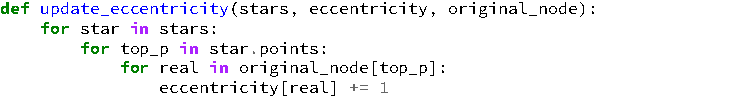
\includegraphics{assets/tmp-code/update_eccentricity.pdf}
    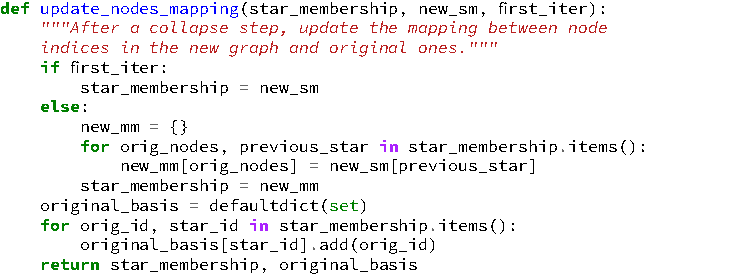
\includegraphics{assets/tmp-code/update_nodes_mapping.pdf}
    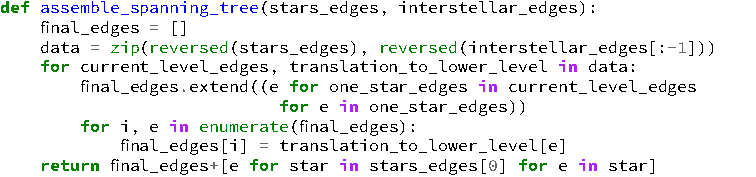
\includegraphics{assets/tmp-code/assemble_spanning_tree.pdf}
	\end{algorithmic}
\end{algorithm}

As described in \autoref{alg:gtx}, \marginpars{I didn't write pseudo code for the three helping functions but
instead put their verbatim python version. They are mostly plumbing code, the only interesting
aspect is their complexity.  \texttt{update\_centrality} and \texttt{update\_nodes\_mapping} takes
$O(n_0)$ time since they go through every node of the original graph. As for
\texttt{assemble\_spanning\_tree}, it goes again through every edges visited at every level of
contraction, meaning it's $O(Tm)$. However, we already visited those edges at least once so it only
adds a constant factor $2$ in the overall complexity of the \gtx{} algorithm.} 
at every contraction level, we first extract stars from the current graph (line 5), then
update the eccentricity and nodes mapping (lines 7--8) and finally contract the graph (line 9) We
perform these operations until there are no edge connecting stars anymore. At this point, we revisit
every outer edges to form the spanning tree (line 13). Because the main loop does not perform any
work besides calling other function, assuming there are $T$ contract steps, the complexity of \gtx{}
is $O(T(m+n)) = O(Tm)$.

Later we hope to found an upper bound of $T$ in terms of $m$, and also to refine the analysis to
leverage the fact that $\sum_{t=0}^T |E_t|$ is significantly smaller than $Tm$. For now, let us
prove the termination of \gtx{} by observing that, assuming $|E_t|>0$, $|E_{t+1}| < |E_t|$ since
at least two nodes in $G_t$ are connected and will therefore form a star, which will remove all the
inner edges of that star. As for the fact that we get a tree, note that a star is a tree, therefore
a star of star is a tree, and so on.\Todo{make the two arguments about \gtx{} correctness more
formal, and also explain that since all nodes are part of the ultimate star, this tree is a spanning
one. Motivate the name of \gtx{}.}

\paragraph{Exemple of \gtx{}}
\label{par:exemple_of_gtx}

We illustrate the operation of the \gtx{} algorithm on small (and somewhat contrived) example.
Let us start with the initial graph $G_0$ depicted in \autoref{fig:gtx_eccentricity}
\vpageref{fig:gtx_eccentricity} and initialize
the eccentricity of all nodes to $0$. When running \extractStar{}, we see that the maximum degree is
$4$, achieved at nodes $\{1, 6, 11, 16, 21, 26, 31, 36, 41\}$. For the sake of simplicity, assume
nodes are picked according to their index. First, node $1$ is forms the star
$\textcolor{DodgerBlue}{S_1^1}$ with peripheral nodes $2$, $3$, $4$ and $5$. This increments the
eccentricity of those peripheral nodes by $1$. Then node $6$ forms its star
$\textcolor{DodgerBlue}{S_2^1}$ with $7$, $8$, $9$ and $10$. The process continues until node $41$ is
chosen to be the center of star $\textcolor{DodgerBlue}{S_9^1}$, at which point the max-priority
queue has been exhausted and \extractStar{} finishes.

\begin{figure}[htbp]
  \centering
  \includegraphics[width=0.78\linewidth]{tikz/gtx_eccentricity_tikz.pdf}
  \caption[The hierarchical structure of stars created by \gtx{}]{%
    The execution of the \gtx{} algorithm. The original graph is made of the solid and dashed edges
    connecting the nodes labeled by their index. Edges forming the final spanning tree are solid
    while the others are dashed. Their colors indicate at which iteration they were chosen to be inside a
    star. The four shades of gray, from white to dark gray
    denote increasing node eccentricity (as computed at the end of the algorithm). The \ith{} star
    created during the \jth{} iteration of the algorithm is denoted $S_i^j$. Refer to the main text
    for the complete description of the execution.}
  \label{fig:gtx_eccentricity}
\end{figure}

\begin{figure}[bthp]
  \centering
  \begin{subfigure}[b]{0.47\textwidth}
    \centering
    \includegraphics[height=5cm]{tikz/gtx_run_level1_tikz}
    \caption{Resulting graph after the first iteration}\label{fig:gtx_run1}
  \end{subfigure}~
  \begin{subfigure}[b]{0.47\textwidth}
    \centering
    \includegraphics[height=2.2cm]{tikz/gtx_run_level2_tikz}
    \caption{Resulting graph after the second iteration}\label{fig:gtx_run2}
    \vspace{\baselineskip}
    \includegraphics[height=2.2cm]{tikz/gtx_run_level3_tikz}
    \caption{Resulting graph after the third iteration}\label{fig:gtx_run3}
  \end{subfigure}~
  \caption{The other iterations of \gtx{}}\label{fig:gtx_run}
\end{figure}

We then call \contractStar{}, with the eccentricity reducing variant. This will connect all possible
pairs of star. For instance, the edge between nodes $19$ and $29$ leads to the edge
between $\textcolor{DodgerBlue}{S_4^1}$ and $\textcolor{DodgerBlue}{S_6^1}$. This is actually the
only possible edge between $\textcolor{DodgerBlue}{S_4^1}$ and $\textcolor{DodgerBlue}{S_6^1}$.
Consider on the other hand the case of edges $(2, 6)$ and $(2, 9)$. They both connect
$\textcolor{DodgerBlue}{S_1^1}$ and $\textcolor{DodgerBlue}{S_2^1}$. Yet at this point of the algorithm,
the eccentricity of node $2$ is $1$, the eccentricity of node $6$ is $0$ and the eccentricity of node
$9$ is $1$. The edge $(2, 6)$ has therefore the smallest total eccentricity and is chosen to connect
$\textcolor{DodgerBlue}{S_1^1}$ and $\textcolor{DodgerBlue}{S_2^1}$. The full result of the
\contractStar{} procedure is $G_1$, which can be seen on \autoref{fig:gtx_run1}.

We now run \extractStar{} on $G_1$. Because all nodes have degree $2$, they could all be chosen to
be the center of a star yet we again consider them ordered by their index and therefore choose
$\textcolor{DodgerBlue}{S_1^1}$ to be the center of the star $\textcolor{Orange}{S_1^2}$ with
peripheral nodes $\textcolor{DodgerBlue}{S_2^1}$ and $\textcolor{DodgerBlue}{S_3^1}$. The original
nodes belonging to those peripheral stars (nodes $4$ to $15$) have their eccentricity incremented by
$1$. The next node with highest degree in $G_1$ is now $\textcolor{DodgerBlue}{S_4^1}$, which forms
a star with $\textcolor{DodgerBlue}{S_5^1}$ and $\textcolor{DodgerBlue}{S_6^1}$. This choice means
that nodes $21$ through $30$ have their eccentricity incremented by $1$. Finally,
$\textcolor{DodgerBlue}{S_7^1}$ forms the last star with $\textcolor{DodgerBlue}{S_8^1}$ and
$\textcolor{DodgerBlue}{S_9^1}$. Then \contractStar{} connects the resulting three stars, and this
time there is only a single choice between each pair of stars, leading to the graph $G_2$ showed in
\autoref{fig:gtx_run2}

The action of \extractStar{} on $G_2$ is quite simple, because there is only one star that can be
created, so let say we choose $\textcolor{Orange}{S_1^2}$ as its center, with
$\textcolor{Orange}{S_2^2}$ and $\textcolor{Orange}{S_3^2}$ as peripheral nodes.  This increases the
eccentricity of their underlying $G_0$ nodes by $1$ (namely nodes $16$ to $45$).  Because there is
only one star $\textcolor{Green}{S_1^3}$ left, \contractStar{} returns $G_3$ showed in
\autoref{fig:gtx_run3} and an empty list of outer edges, meaning that the inner loop of \gtx{} is
finished and we can go through every edges we chose between stars at every level to recover the
final spanning tree, showed with black edges in \autoref{fig:gtx_eccentricity}
\vpageref{fig:gtx_eccentricity}. For completeness, we can also look at the edges which are not part
of the spanning tree and therefore contribute to the stretch of the tree. In that case the average
stretch is $7$, as showed in \autoref{tab:gtx_example_stretch}.

\begin{table}[htpb]
  \centering
  \caption{Stretch of the example tree}
  \label{tab:gtx_example_stretch}
  \begin{tabulary}{\linewidth}{lLr}
    \toprule
    test edge & path in the tree & length \\
    \midrule
    $2,9$   & $2$--$6$--$9$                       & $2$ \\
    $3,12$  & $3$--$1$--$4$--$14$--$11$--$12$     & $6$ \\
    $13,29$ & $13$--$11$--$15$--$26$--$29$        & $4$ \\
    $20,24$ & $20$--$16$--$17$--$23$--$21$--$24$  & $5$ \\
    $25,42$ & $25$--$21$--$23$--$17$--$16$--$19$--$29$--$26$--$15$--$11$--$14$--$4$--$1$--$2$--$6$--$8$--$37$--$36$--$39$-- $32$--$31$--$35$--$43$--$41$--$45$ & $24$ \\
    $33,38$ & $33$--$31$--$32$--$39$--$36$--$38$  & $5$ \\
    $34,43$ & $34$--$31$--$35$--$43$              & $3$ \\
    \bottomrule
  \end{tabulary}
\end{table}

\paragraph{Number of iterations needed}\label{par:number_of_iteration}%

\textcolor{red}{\LARGE Draft}

A crucial quantity of the \gtx{} algorithm, both in terms of complexity and resulting stretch, is
the number of contraction $T$ needed before termination. While this is still elusive to express in the
general case, let us first look at some simple cases. For instance, a very sparse example of graph
is the line graph. While it is already a tree, let us look how the \gtx{} algorithm operates on it.
Say we have $n$ nodes in that line. There a star is made at most of three consecutive nodes. In the
worst case, centers will be chosen such that we have a succession of three and two nodes stars (as
in \autoref{fig:gtx_line_graph}).%
\begin{marginfigure}
  \centering
  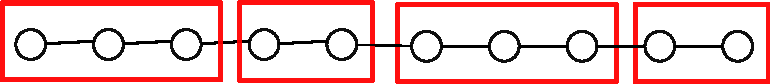
\includegraphics[width=0.9\linewidth]{assets/tmp-code/line_graph.pdf}
  \caption{A line graph with stars in red}
  \label{fig:gtx_line_graph}
\end{marginfigure}
This will results in $\nicefrac{2n}{5}$ stars, which is less than half of $n$ and because in that
case $n\approx m$, \gtx{} will finish after $O(\log m)$ iterations. Note that a barbell graph (two
cliques connected by a line) would require a number of iterations proportional to the length of that
central line, despite having many more edges. This suggests unsurprisingly that the diameter of the graph
could be a good parameter to quantify the number of iteration needed. Indeed, take a tree a consider
the length $p$ of its longest path from the root to a leaf. By a similar argument as the one used in
the line case, it seems \gtx{} will terminate after $O(\log p)$ iterations.
